\documentclass[a4paper,12pt]{article}
\setcounter{secnumdepth}{2}
\newcommand{\code}[1]{{\footnotesize{{\tt #1}}}}
\usepackage{natbib}
\usepackage{color}
\usepackage{graphicx}
\usepackage{listings}
\lstset{
basicstyle=\small\ttfamily,
columns=flexible,
breaklines=true
}
\addtolength{\textwidth}{2cm} % a = -2b, where this is a and below is b
\addtolength{\hoffset}{-1cm}
\addtolength{\textheight}{2cm} % c = -d, where this is c and d is below
\addtolength{\voffset}{-2cm}
\begin{document}
\title{RIA: Regional IBD Analysis}
\date{}
\author{}
\maketitle
\newpage
\tableofcontents
\newpage
\section{Introduction}
\label{introduction}

The program RIA is a C++ implementation of the method described in \citet{nat:15} and uses calls to programs PLINK and KING version 2.2.9.
\subsection{Overview}
\label{overview}

The program RIA performs the following steps calling external PLINK and KING where required: 
\begin{enumerate}

\item The first stage of RIA is the estimation of the IBD sharing probabilities between affected family members using a selection of SNPs across all available SNPs in the data, these probabilities form the {\it priors}. The program PLINK \citet{purcell:etal:07} is used to prune the SNPs to give a representative selection of SNPs using only founders. Thus, it should be noted that founders are required in the SNP data. The cases are then used to estimate the IBD sharing probabilities using KING (version 2.2.9) \citet{manichaikul:etal:10}. See  section \ref{ibd-calc} on how the IBD sharing probabilities are estimated. 
\item The next stage is to step across the genome, set to a default of 50 SNPs per step, and form a SNP window of around 500 to 2000 SNPs and use these SNPs to estimate the IBD sharing probabilities between affected family members using KING (version 2.2.9). These probabilities give the {\it posteriors}. See  section \ref{ibd-calc} on how the IBD sharing probabilities are estimated. 
\item The next step is to perform a non-parametric linkage analysis comparing the prior and posterior IBD sharing probabilities using the method as described in \citet{cordell:etal:00} with minor modifications as described in \citet{nat:15}. This produces a LOD score for each analysed SNP region together with parameter estimates for the (scaled) additive and dominance variances.\end{enumerate}

For full details of the methodology of RIA please see the accompanying paper \citet{nat:15}. 

%============ End of subsection "overview"============

\subsection{Estimation of IBD sharing probabilities}
\label{ibd-calc}

KING version 2.2.9~is used with option \code{--homog} to estimate the IBD sharing probabilities. Let {\it IBD2}, {\it IBD1} and {\it IBD0} be the probabilities that two individuals share 2, 1 or 0 alleles IBD respectively and {\it K} the kinship coefficient, then {\it IBD2}, {\it IBD1} and {\it IBD0} are estimated for each SNP as follows: 
\begin{enumerate}

\item KING version 2.2.9 is ran with the \code{--homog} option which returns estimates of {\it K} and {\it IBD0}. 
\item {\it K} and {\it IBD0} are truncated to plausible values between 0 to 0.5 and between 0 to 1 respectively if necessary. 
\item {\it IBD2} is estimated as {\it 4K - (1 - IBD0)}. 
\item {\it IBD2} is truncated to a plausible value between 0 to 1 if necessary. 
\item {\it IBD1} is estimated as {\it 1 - IBD0 - IBD2}. 
\item {\it IBD1} is truncated to a plausible value between 0 to 1 if necessary. 
\item For the posterior probabilities only: if any of the priors for {\it IBD2}, {\it IBD1} or {\it IBD0} are equal to zero then the corresponding posterior values are also set to zero. If this results in all IBD probabilities being equal to zero then an error is reported. 
\item {\it IBD2}, {\it IBD1} and {\it IBD0} are scaled so that {\it IBD2 + IBD1 + IBD0 = 1} if necessary.\end{enumerate}

%============ End of subsection "ibd-calc"============


%================== End of section "introduction"==================

\section{Installation}
\label{installation}

Download an executable file from the home~page for your system and off you go, or do the following. 
\begin{enumerate}

\item Download the code from the home page. 
\item Compile it by typing something like the following: \vspace{0.35cm} \begin{lstlisting}
g++ -O3 src/*.cpp -o ria

\end{lstlisting} \vspace{0.35cm}
\item It is also necessary to having working copies of the programs PLINK~and KING version 2.2.9~installed. {\bf Note:} It is very important to download KING version 2.2.9 and not any later versions as we need to use the \code{--homog} option which is no longer available in later versions. 
\item Start analysing your data with RIA! 
\item If you are using Windows then you will need to uncomment the line below in the \code{main.h} file: \vspace{0.35cm} \begin{lstlisting}
#define USING_WINDOWS

\end{lstlisting} \vspace{0.35cm}\end{enumerate}

%================== End of section "installation"==================

\section{Using RIA}
\label{using}

The program RIA takes a PLINK binary file as input (.bed/.bim/.fam) and produces a results file of the analysis. Basic usage of the program is given by typing: 
\vspace{0.35cm} \begin{lstlisting}
./ria -i mydata.bed

\end{lstlisting} \vspace{0.35cm}
The most likely options that will need to be used are how to run the programs PLINK and KING: 
\vspace{0.35cm} \begin{lstlisting}
./ria -plink /home/me/my-programs/plink/plink -king /home/me/my-programs/king/king -i mydata.bed

\end{lstlisting} \vspace{0.35cm}
Typing \code{ria} with no options will output usage details: 
\vspace{0.35cm} \begin{lstlisting}
RIA: Regional IBD Analysis, v1.1
------------------------------------------------------------
Copyright 2015-present Richard Howey, GNU General Public License, v3
Research Software Engineering, Newcastle University

Usage:
  ./ria [options] -i pedigree.bed
 or ./ria -pf parameterfile [pedigree.bed]

Options:
  -window-size-cm n     -- set window size to n centimorgans
  -window-min-snps m    -- set required minimium number of SNPs in a window to m
  -step-size s          -- step size of windows, s
  -start-snp a          -- start analysis from SNP number a
  -end-snp b            -- end analysis at SNP number b
  -start-snp-name x     -- start analysis from SNP name x
  -end-snp-name y       -- end analysis at SNP name y
  -job d t              -- job number d of t
  -i file.bed           -- input binary pedigree file, file.bed
  -o results.dat        -- output results file, results.dat
  -i-prior file         -- input prior IBDs, file
  -o-prior file         -- output prior IBDs, file
  -prior-only           -- calculate prior IBDs only
  -plink command        -- command used to run PLINK
  -plink-options "ops"  -- PLINK pruning options used to calculate the prior
  -king command         -- command used to run KING
  -log results.log      -- log filename, results.log
  -ndv                  -- no dominance variance
  -so                   -- suppress output to screen

Default Options in Effect:
  -window-size-cM 15
  -window-min-snps 100
  -step-size 50
  -plink plink
  -king king
  -o riaResults.dat

\end{lstlisting} \vspace{0.35cm}
See  section \ref{example} for an example of how to use RIA to analyse some data. 
\subsection{Parameter file}
\label{parameterfile}

A parameter file, \code{.pf}, may be used with RIA instead of writing all of the options on the command line. To use a parameter file simply type: 
\vspace{0.35cm} \begin{lstlisting}
./ria -pf myparameters.pf

\end{lstlisting} \vspace{0.35cm}
The parameter file should be a text file with one option written on each line. For example, to perform the analysis above the file \code{myparameters.pf} would be as follows: 
\vspace{0.35cm} \begin{lstlisting}
-plink /home/me/my-programs/plink/plink
-king /home/me/my-programs/king/king mydata.bed
-window-size-cm 15
-step-size 50
-i mydata.bed
-o myResults.dat

\end{lstlisting} \vspace{0.35cm}
It is also possible to add comments to the file provided that the ``-'' character is not used, and to comment out any options by placing another character in front of any ``-''. For example, the above parameter file could be edited as follows: 
\vspace{0.35cm} \begin{lstlisting}
# Command used to run PLINK
-plink /home/me/my-programs/plink/plink

# Command used to run KING
-king /home/me/my-programs/king/king

# SNP window size
-window-size-cm 15

# Number of SNPs to move to the next SNP window
-step-size 50

# The all important data to analyse
-i mydata.bed

# My lovely analysis results
-o myResults.dat

# I might try this later
#-i myOtherData.bed

\end{lstlisting} \vspace{0.35cm}
%============ End of subsection "parameterfile"============

\subsection{Temporary Files}
\label{temporary}

RIA requires the use of two other programs, PLINK and KING, and in order to use these programs several temporary files must be created. All of these files begin with ``tempRIA'' and, before the file extension, end with the process ID of the current RIA job. They will typically appear similar to the following: 
\vspace{0.35cm} \begin{lstlisting}
tempRIA-priors1-57703.prune.in
tempRIA-priors2-57703.bed
tempRIA-priors2-57703.bim
tempRIA-priors2-57703.fam
tempRIA-priors2-57703.kin
tempRIA-post-57703.fam
tempRIA-posterior-57703.bed
tempRIA-posterior-57703.bim
tempRIA-posterior-57703.fam
tempRIA-posterior-57703.kin

\end{lstlisting} \vspace{0.35cm}
The use of the process ID ensures that several RIA jobs may be ran in the same location without any issues of interference. All of these temporary files should be deleted by RIA when they are no longer needed, however if RIA is forced to unexpectedly stop for some reason then these files may still be lying around. In which case, they should be carefully deleted if necessary. 

%============ End of subsection "temporary"============


%================== End of section "using"==================

\section{RIA Example}
\label{example}

This section runs through an example analysis using RIA with example data which can be download from here.This data was simulated using HAPMAP3 data to mate individuals who already had children to create 301 affected relative pairs (ARPs). The data only contains SNPs from chromosome 6, however in a real analysis we would ideally have data for the whole genome to get better estimates of the prior IBD sharing probabilities and to compare LOD scores across the genome. 

We already have PLINK installed on our system so we will not bother ourselves to download it from here,~nor will we use the \code{-plink} option as it is already set up to run by typing ``plink'', which is set by default. The KING program (version 2.2.9) on the other hand is not installed, so we shall download it from here,~and save the executable file at location \code{/home/me/my-programs/king/} so that KING may be ran by typing \code{/home/me/my-programs/king/king}. {\bf Note:} It is very important to download KING version 2.2.9 and not any later versions as we need to use the \code{--homog} option which is no longer available in later versions. 

We can now run a Regional IBD Analysis (RIA) analyses using the default options for the SNP window size, set to 15 cM, and the SNP window step size, set to 50, by typing: 
\vspace{0.35cm} \begin{lstlisting}
./ria -king /home/me/my-programs/king/king -i exampleRIAData.bed -o resultsRIAExample.dat

\end{lstlisting} \vspace{0.35cm}
This will create output similar to the following. 
\vspace{0.35cm} \begin{lstlisting}
RIA: Regional IBD Analysis, v1.1
------------------------------------------------------------
Copyright 2015-present Richard Howey, GNU General Public License, v3
Research Software Engineering, Newcastle University

Parameters:
Input file: demo-data/exampleRIAData.bed
Output file: resultsRIAExampleDataKing2023.dat
Log file: resultsRIAExampleDataKing2023.log
Using additive and dominance variance model
Start at first SNP with full SNP window
End at last SNP with full SNP window
Window size: 15 cM
Minimum number of SNPs in a window: 100
SNP step size: 50 SNPs
Number of cases: 362
Number of unused controls: 35
Number of SNPs: 29413

Creating list of pruned SNPs using PLINK command:
plink --noweb --indep 50 50 2 --mind 0.01 --maf 0.25 --geno 0.05 --bfile exampleRIAData --out tempRIA-priors1-8553 >/dev/null 2>&1

Creating data file to calculate priors using PLINK command:
plink --noweb --bfile exampleRIAData --filter-cases --extract tempRIA-priors1-8553.prune.in --make-bed --out tempRIA-priors2-8553 >/dev/null 2>&1

Calculating priors using KING command:
/home/me/my-programs/king/king -b tempRIA-priors2-8553.bed --homog --prefix tempRIA-priors2-8553 >/dev/null 2>&1

Number of affected relative pairs (ARPs) in priors: 301

Calculating posteriors (for each SNP window) using KING command:
/home/me/my-programs/king/king -b tempRIA-posterior-8553.bed --homog --prefix tempRIA-posterior-8553 >/dev/null 2>&1

15 cM windows - number of SNPs summary statistics:
Mean: 2442.33
Median: 2266
Standard deviation: 606.466
Range: (1458, 3634)

Run time: 10 minutes

\end{lstlisting} \vspace{0.35cm}
The commands used by PLINK and KING are output for reference and may be useful if there are any problems. RIA uses several intermediate temporary files beginning with ``tempRIA'' and may be lying around if there was a problem and RIA was forced to unexpectedly stop. They should then be carefully deleted if necessary. 

The results file \code{resultsRIAExample.dat} should look as follows: 
\vspace{0.35cm} \begin{lstlisting}
SNP CHR ID CM BP VAR_A VAR_D MLS
741 6 rs11755767 7.52007 2804601 1.583936049 0 2.828838716
791 6 rs7765538 8.14908 3000876 1.544010298 0 2.726726528
841 6 rs744375 8.85487 3294907 1.473726461 0 2.565180586
891 6 rs7763703 9.47382 3433624 1.392624092 0 2.383495002
941 6 rs12526106 10.0032 3690722 1.339150984 0 2.272297645
...
28341 6 rs11755875 188.372 166136328 1.21271465 0.1564407936 2.774211867
28391 6 rs705791 188.972 166288440 1.127065043 0.1950593781 2.693304349
28441 6 rs12154075 189.175 166486261 1.12910064 0.1965589048 2.69542933
28491 6 rs1033725 189.362 166627240 1.125312283 0.1817039321 2.647993295
28541 6 rs6935542 190.191 166817722 0.9200496884 0.3786320582 2.675835187

\end{lstlisting} \vspace{0.35cm}
The columns for the results file are as follows: 

{\begin{center}\begin{tabular}{ll}
Column  & Description\\
\hline
SNP  & The SNP number as it appears in file.\\
CHR  & Chromosome of the SNP.\\
ID  & The name of the SNP.\\
CM  & The centimorgan value of the SNP.\\
BP  & The base pair position of the SNP.\\
VAR\_A & The additive variance parameter.\\
VAR\_D & The dominance variance parameter.\\
MLS  & The maximum-likelihood statistic.\\
\end{tabular}\end{center}}

It is not unusual for either VAR\_A~or VAR\_D~or even both of these parameters to be equal to 0. In the example data set VAR\_D~is equal to 0 for most of the SNPs. 

In R type: 
\vspace{0.35cm} \begin{lstlisting}
resultsRIAExample<-read.table("resultsRIAExample.dat", header=TRUE)

plot(resultsRIAExample$BP/10^6, resultsRIAExample$MLS, main="Regional IBD Analysis", xlab=expression(bp~position~(Mb)), ylab="MLS", ylim=c(0, max(resultsRIAExample$MLS)))

\end{lstlisting} \vspace{0.35cm}
This will produce the following plot: 
{\begin{figure}[ht]
{\begin{center}
{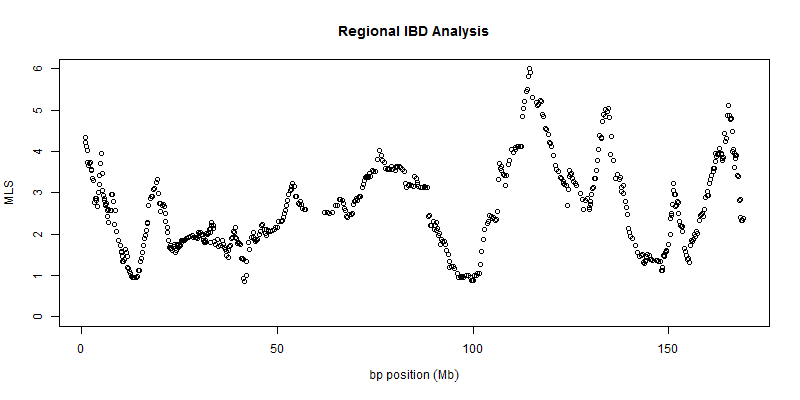
\includegraphics[width=400pt]{exampleRIA.png}}
\caption{Plot of RIA test results.}
\label{example-fig}
\end{center}}
\end{figure}
}

As the prior IBD sharing probabilities are always the same, regardless of which subset of SNPs are analysed, it is possible to save a prior file using the \code{-o-prior} option as follows 
\vspace{0.35cm} \begin{lstlisting}
./ria -king /home/me/my-programs/king/king -i exampleRIAData.bed -o resultsRIAExample.dat -o-prior examplePrior.dat

\end{lstlisting} \vspace{0.35cm}
or can be done without any further analysis using the \code{-prior-only} option as follows 
\vspace{0.35cm} \begin{lstlisting}
./ria -king /home/me/my-programs/king/king -i exampleRIAData.bed -prior-only -o-prior examplePrior.dat

\end{lstlisting} \vspace{0.35cm}
The prior can then be used for different analysis using the \code{-i-prior} option, such as 
\vspace{0.35cm} \begin{lstlisting}
./ria -window-size 2000 -king /home/me/my-programs/king/king -i exampleRIAData.bed -o resultsRIAExample-2000.dat -i-prior examplePrior.dat

\end{lstlisting} \vspace{0.35cm}
There are no simulated effects in the example data, which would be clearer if results for the whole genome were available. For details on how to interpret results please see \citet{nat:15}. 
\subsection{Parallel processing}
\label{parallel}

Regional IBD Analysis is fairly computationally intensive and so it is natural to want to speed things up a bit by using parallel processing. This can be done by dividing the analysis up using the \code{-start-snp} and \code{-end-snp} options, such as 
\vspace{0.35cm} \begin{lstlisting}
./ria -king /home/me/my-programs/king/king -i exampleRIAData.bed -o resultsRIAExample1.dat -i-prior examplePrior.dat -start-snp 3000 -end-snp 4000

\end{lstlisting} \vspace{0.35cm}
Care must be taken when setting the first SNP to ensure there is a full SNP window around the SNP at the center of the SNP window. 

If all of the data is to be analysed it is much easy to use the \code{-job} option to divide the analysis into a number of analyses. This will automatically set the start and end SNPs. For example, to analyse all of the data in 10 jobs using the previously calculated priors, use 
\vspace{0.35cm} \begin{lstlisting}
./ria -king /home/me/my-programs/king/king -i exampleRIAData.bed -o results1.dat -i-prior examplePrior.dat -job 1 10
./ria -king /home/me/my-programs/king/king -i exampleRIAData.bed -o results2.dat -i-prior examplePrior.dat -job 2 10
./ria -king /home/me/my-programs/king/king -i exampleRIAData.bed -o results3.dat -i-prior examplePrior.dat -job 3 10
./ria -king /home/me/my-programs/king/king -i exampleRIAData.bed -o results4.dat -i-prior examplePrior.dat -job 4 10
./ria -king /home/me/my-programs/king/king -i exampleRIAData.bed -o results5.dat -i-prior examplePrior.dat -job 5 10
./ria -king /home/me/my-programs/king/king -i exampleRIAData.bed -o results6.dat -i-prior examplePrior.dat -job 6 10
./ria -king /home/me/my-programs/king/king -i exampleRIAData.bed -o results7.dat -i-prior examplePrior.dat -job 7 10
./ria -king /home/me/my-programs/king/king -i exampleRIAData.bed -o results8.dat -i-prior examplePrior.dat -job 8 10
./ria -king /home/me/my-programs/king/king -i exampleRIAData.bed -o results9.dat -i-prior examplePrior.dat -job 9 10
./ria -king /home/me/my-programs/king/king -i exampleRIAData.bed -o results10.dat -i-prior examplePrior.dat -job 10 10

\end{lstlisting} \vspace{0.35cm}
The temporary intermediate files used by RIA depend on the process ID of each job so there is no need to worry about these files interfering with one another. Only the first results file will contain the header making it easy to combine the results into one results file: 
\vspace{0.35cm} \begin{lstlisting}
cat results1.dat results2.dat results3.dat results4.dat results5.dat results6.dat results7.dat results8.dat results9.dat results10.dat > allResults.dat

\end{lstlisting} \vspace{0.35cm}
The \code{-job} option makes it easy to write a simple script with a loop to submit the jobs. Alternatively, if you are using a High Performance Computing (HPC) cluster using the open-source Sun Grid Engine (SGE) scheduler software, then these jobs may be submitted as an array job using something similar to the following script: 
\vspace{0.35cm} \begin{lstlisting}
#!/bin/bash
# execute in current working directory
#$ -cwd
# export local envirnoment
#$ -V
# the number of RIA tasks
#$ -t 1-10
# execute RIA for each task
./ria -king /home/me/my-programs/king/king -i exampleRIAData.bed -o results$SGE_TASK_ID.dat -i-prior examplePrior.dat -job $SGE_TASK_ID 10

\end{lstlisting} \vspace{0.35cm}
%============ End of subsection "parallel"============


%================== End of section "example"==================

\bibliographystyle{genepi}
\bibliography{../../../work-other/tex/biblio}
\end{document}